\documentclass{beamer}
\usepackage{beamerthemesplit} % new 
\usepackage[utf8x]{inputenc}
\usepackage[ngerman]{babel} 

\usepackage{epsfig}
\usepackage{amsmath}
\usepackage{placeins}
\usepackage{float}

\usepackage{algorithmic}
\usepackage[linesnumbered,ruled,vlined]{algorithm2e}


\begin{document}
\title{A Hybrid Algorithm for the Partition Coloring Problem} 
\author{Gilbert Fritz} 
\date{\today} 

\frame{\titlepage} 

\frame{\frametitle{Table of contents}\tableofcontents} 


\section{Problem Description} 
\subsection{Partition Coloring Problem}
\frame{\frametitle{Partition Coloring Problem}
\begin{itemize}
\item given $G = (V, E)$
\item let $V_1, V_2,\ldots, V_q$ be a partition of $V$ into $q$ disjoint subsets
\item find a subset $V' \subset V$ such that $|V' \cap V_i| = 1, \forall i = 1, \ldots , q$ (i.e., $V'$ contains one
node from each component $V_i$)
\item find a coloring on the induced graph, such that the chromatic number of the graph induced in $G$ by $V'$ is minimum.  \item Proof of Li and Simha has shown that PCP is $\mathcal{NP}$-complete.
\end{itemize}
}
\frame{\frametitle{Partition Coloring Problem}
\begin{center}
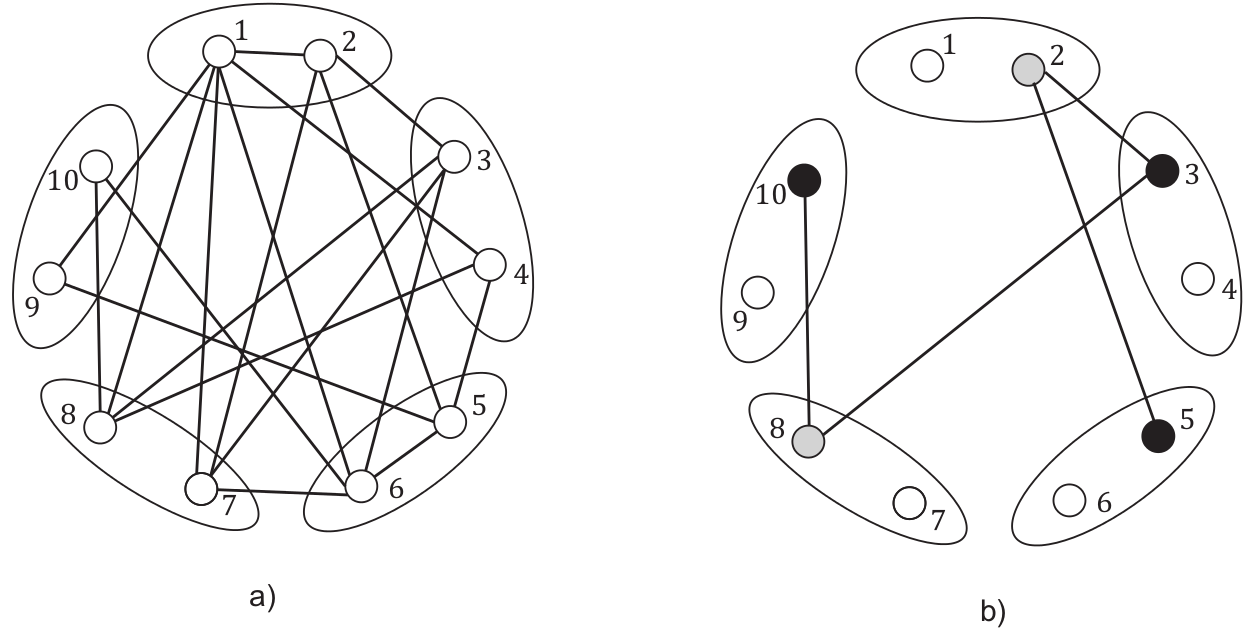
\includegraphics[scale=0.3]{pcp.png}
\end{center}
}

\subsection{Application to min-RWA}
\frame{\frametitle{Routing and Wavelength Assignment}
\begin{itemize}
\item Finding paths
\item Assigning Wavelengths is dual to PCP
\end{itemize}
\begin{center}
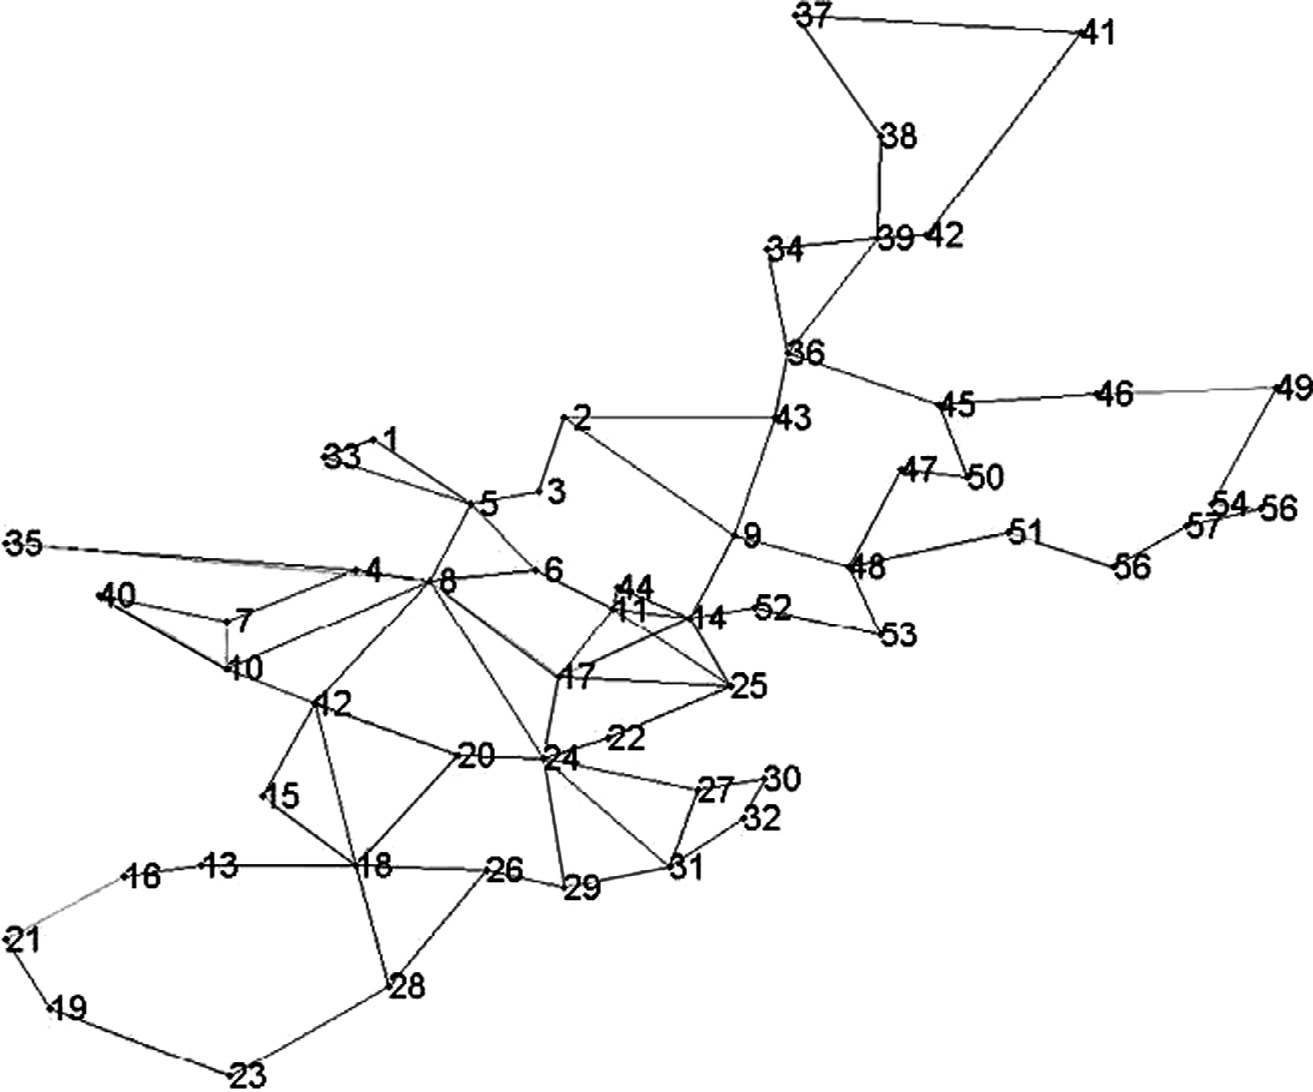
\includegraphics[scale=0.18]{rwa.png}
\end{center}
}


%TODO noch mehr über alle papers schreiben
\section{Previous Works} 
\frame{
\frametitle{Previous Works}
Exact:
\begin{enumerate}
\item Frota, Ribiero (2010): Branch-And-Cut %algorithm based on a formulation by representative vertices
\item Hoshino, Souza, Frota (2011): Branch-And-Price
\end{enumerate}
Heuristics:
\begin{enumerate}
\item Li, Shima (2000): Group of heuristics based on extensions of classical methods for the vertex coloring problem
\item Noronha, Ribiero (2006): Tabusearch
\item Hu, Raidl, Pop (2013): Memetic algorithm
\end{enumerate}
}

\section{My Approach}
\subsection{Overview}
\frame{\frametitle{Algorithm Overview}
\begin{enumerate}
\item Create initial solution: OneStepCD
\item For each set $U$ of vertices of same color $c$: recolor without using $c$ by $\{RANDOM, OneStepCD, ILP1, ILP2\}$
\item Sort the solutions by amount of conflicts.
\item For each solution try to eliminate conflicts by using tabusearch. Put each vertex-color-pair on the tabulist for a specified amount of iterations. 
\item If all the conflicts could be eliminated, go back to 2, else return the latest feasible solution.
\end{enumerate}
}

\subsection{Initial Solution}
\begin{frame}
\frametitle{Initial Solution: OneStepCD}
  \begin{algorithm}[H]
  \scriptsize
  \KwIn{An uncolored Graph $G=(V,E)$}
  \KwOut{A feasible Coloring $V'$}
  Remove from G all edges $(i,j) \in E$ : $i,j \in V_k$ for some $k=1,\ldots,q$\; 
  Set $V' \gets \emptyset $\;
  \While{$|V'| < q$} {
    Set $X \gets \emptyset $\;
    \For{$k=1,\ldots,q$ : $V_k \cap V'=0$}{
      Set $X \gets X \cup argmin\{CD(i) : i \in V_k\}$\; 
    }
    Set $x \gets argmax\{CD(i) : i \in X \}$\;
    Set $V' \gets V' \cup \{x\}$\;
    Assign the minimum possible colour to x\;
    Remove from G all nodes in $V_{c(x)} \setminus \{x\} $\;
  }
  \Return{$V'$}\;
  \caption{{\sc OneStepCD}}
  \label{algo:osdc}
  \end{algorithm}
\end{frame}

\FloatBarrier
\subsection{Reselecting/Recoloring subgraphs}
\begin{frame}
\frametitle{Random Recoloring}
\begin{enumerate}
\item Nodes are reselected and recolored randomly.
\end{enumerate}

\end{frame}

\frame{\frametitle{Recoloring with OneStepCD}
\begin{algorithm}[H]
\scriptsize
\KwIn{A partial Solution $P$, a number of maximum colours $cmax$ }
\KwOut{A feasible Solution $S$}
Let $U$ be the set of uncolored nodes in $P$\;
Set $S \gets \emptyset$\;
\While{$|U| > 0$} {
  Set $X \gets \emptyset $\;
  \For{ $u \in U$}{
    $X \gets X \cup argmin\{CD(i) : i \in V_{c(u)}\}$\; 
  }
  Set $x \gets argmax\{CD(i) : i \in X \}$\;
  Set $cmin \gets$ the minimum possible colour that can be assigned to x\;
  \If{$cmin \geq cmax$}{
    $cmin \gets$ the color that produces the fewest conflicts.
  }
  Assign $cmin$ to $x$\;
  $S \gets S \cup \{x\}$\;
  $U \gets U \setminus V_{c(x)}$\;
}
\Return{$V'$}\;
\caption{{\sc OneStepCD Recoloring}}
\label{algo:osdc2}
\end{algorithm}
}
\frame{\frametitle{Recoloring with ILP1}

Let $Q = {Q_1,\ldots,Q_q}$ be the set of Clusters. Every cluster $Q_p$ consists of a set of nodes. Let $C=\{1,\ldots,cmax\}$ be the
set of allowed colors. Let $M$ be a 3-dimensional array of constants, storing
for every cluster $p \in Q$, the number conflicts that would occur by selecting the pair $(v \in Q_p, c \in C)$.
$E$ denotes the set of edges and $P[v]$ the cluster of node $v$.


\begin{equation*}
\scriptsize
\begin{aligned}
& \underset{X}{\text{minimize}} && \sum_{p \in Q}\sum_{v \in Q_p}\sum_{c \in C} X_{pvc} * M_{pvc}                    &&&(1)\\
& \text{subject to} && \sum_{v \in Q_p}\sum_{c \in C} X_{pvc}=1, && \forall p \in Q    &(2)\\
&&& X_{pvc}+X_{quc} \leq 1, && \forall ((p,v),(q,u)) \in E, \forall c \in C     &(3)\\
&&& X_{pvc} \in \{0,1\}, && \forall p \in Q, \forall v \in Q_p, \forall c \in C         &(4)
\end{aligned}
\end{equation*}
}


\frame{\frametitle{Recoloring with ILP2}

Let $U$ be the set of uncolored nodes in uncolored clusters and $color[(p,v)]$ the color of the node $v$ in partition $p$.

\begin{equation*}
\scriptsize
\begin{aligned}
& \underset{Z}{\text{minimize}} && \sum_{p \in Q}\sum_{v \in Q_p}\sum_{c \in C} Z_{pvc}                                              &&&(1)\\
& \text{subject to} && Z_{pvc} \geq X_{quc}, && \forall ((p,v),(q,u))\in E : (p,v) \notin U, (q,u) \in U,\\&&&&& c=color[(p,v)]                                                            &(2)\\
&&& \sum_{v \in Q_p}\sum_{c \in C} X_{pvc}=1, && \forall p \in Q   &(3)\\
&&& X_{pvc}+X_{quc} \leq 1, && \forall ((p,v),(q,u)) \in E, \forall c \in C     &(4)\\
&&& X_{pvc} \in \{0,1\}, && \forall p \in Q, \forall v \in Q_p, \forall c \in C        &(5)
\end{aligned}
\end{equation*}

}

\subsection{Eliminating Conflicts: Tabusearch}
\begin{frame}[fragile]
\frametitle{Tabusearch: Outline}
\begin{enumerate}
\item Let $R$ be the set of clusters that has been recolored before.
\item Initialize $C$ with the set of conflicting clusters not in $R$.
\item Over all cluster in $C$, search for the node-color pair $(n,c)$ that produces the fewest conflicts and is not on the tabulist.
\item Select and color node $n$ with color $c$ and add $(n,c)$ to the tabulist.
\item Remove the cluster of node $n$ from $C$.
\item Add the clusters of all the produced conflicting nodes to set $C$.
\item If $C$ is not empty, go back to step 3.
\end{enumerate}
\end{frame}

%TODO resultate besser darstellen und vergleichen
\section{Results}
\subsection{Instances and Testing Environment}

\frame{\frametitle{Instances and Testing Environment}
\begin{enumerate}
%\item Instances of Noronha, Ribiero
%
%\begin{center}
%\begin{tabular}{|c|c|c|c|c|}
%\hline
%\textbf{Instance} & \textbf{Nodes} & \textbf{Clusters} & \textbf{N/Cl} & \textbf{Density} \\
%\hline
%dsjc500.5-1.in & 500 & 500 & 1 & 0.5\\
%\hline
%dsjc500.5-2.in & 1000 & 500 & 2 & 0.5\\
%\hline
%dsjc500.5-3.in & 1500 & 500 & 3 & 0.5\\
%\hline
%dsjc500.5-4.in & 2000 & 500 & 4 & 0.5\\
%\hline
%\end{tabular}
%\end{center}


\item Java implementation
\item System: Intel i5 DualCore 2.5GHz
\end{enumerate}
}

\frame{

\begin{table}
\frametitle{Instances with different size: Conflicting Nodes}
\resizebox{\columnwidth}{!}{%

\begin{tabular}{|l|l||l||l||l||l|}
\hline
\multicolumn{2}{|l||}{Instance set}&\multicolumn{1}{l||}{Random (10 runs/inst)}&\multicolumn{1}{|l||}{OneStepCD}&\multicolumn{1}{|l||}{ILP1}&\multicolumn{1}{|l|}{ILP2}\\
\cline{1-6}
 nodes & density   & $\overline{cnodes/recoloring}$  & $\overline{cnodes/recoloring}$ & $\overline{cnodes/recoloring}$ & $\overline{cnodes/recoloring}$\\
\hline
20 & 0.5 & 		3.694   & 2.25  	& 1.605  	& 1.363\\
40 & 0.5 & 		7.338    & 3.854  & 3.215	  & 2.295\\
60 & 0.5 & 		10.218    & 4.99   & 4.218	  & 2.834\\
70 & 0.5 & 		11.3    & 5.845	  	& 4.563	  	& 3.274\\
80 & 0.5 & 		12.696    & 6.048	 & 4.979 	& 3.415\\
90 & 0.5 & 		12.324    & 5.93	  & 4.648	  & 3.387\\
100 & 0.5 & 	14.914    & 7.1		  & 5.235	  & 3.926\\
120 & 0.5 & 	15.530    & 6.447	  & 5.078	  & 3.386\\
\hline
\end{tabular}
}
\end{table}
}


\frame{

\begin{table}
\frametitle{Instances with different size: Results}
\resizebox{\columnwidth}{!}{%

\begin{tabular}{|l|l||l|l|l||l|l|l||l|l|l||l|l|l|}
\hline
\multicolumn{2}{|l||}{Instance set}&\multicolumn{3}{l||}{Random (10 runs/inst)}&\multicolumn{3}{|l||}{OneStepCD}&\multicolumn{3}{|l||}{ILP1}&\multicolumn{3}{|l|}{ILP2}\\
\cline{1-14}
 nodes & density   & $\overline{obj}$ & $sd$ & $\overline{time}$  & $\overline{obj}$ & $sd$ & $\overline{time}$  & $\overline{obj}$ & $sd$ & $\overline{time}$  & $\overline{obj}$ & $sd$ & $\overline{time}$\\
\hline
20 & 0.5   & \textbf{3.0} & 0.0 & 0.015   & \textbf{3.0} & 0.0 & 0.07  & \textbf{3.0} & 0.0 & 0.113  & \textbf{3.0} & 0.0 & 0.123\\
40 & 0.5   & \textbf{4.0} & 0.0 & 0.023   & \textbf{4.0} & 0.0 & 0.053  & \textbf{4.0} & 0.0 & 0.148   & \textbf{4.0} & 0.0 & 0.224\\
60 & 0.5   & \textbf{5.0} & 0.0 & 0.061   & \textbf{5.0} & 0.0 & 0.098  & \textbf{5.0} & 0.0 & 0.251   & \textbf{5.0} & 0.0 & 0.473\\
70 & 0.5   & \textbf{6.0} & 0.0 & 0.081   & \textbf{6.0} & 0.0 & 0.086  & \textbf{6.0} & 0.0 & 0.214   & \textbf{6.0} & 0.0 & 0.479\\
80 & 0.5   & \textbf{6.27} & 0.137 & 0.153  & \textbf{6.2} & 0.159 & 0.186  & \textbf{6.2} & 0.159 & 0.340   & \textbf{6.2} & 0.159 & 0.755\\
90 & 0.5   & \textbf{7.884} & 15.478 & 0.369  & \textbf{7.911} & 15.547 & 0.384 & \textbf{7.888} & 15.52 & 0.597   & \textbf{7.91} & 15.547 & 1.084\\
100 & 0.5   & \textbf{7.12} & 0.013 & 0.326   & \textbf{7.2} & 0.159 & 0.323  & \textbf{7.2} & 0.159 & 0.53   & \textbf{7.0} & 0.0 & 1.395\\
120 & 0.5   & \textbf{8.64} & 0.198 & 0.521   & \textbf{8.6} & 0.24 & 0.644  & \textbf{8.6} & 0.24 & 0.858   & \textbf{8.6} & 0.24 & 1.859\\
\hline
\end{tabular}
}
\end{table}
}

\frame{

\begin{table}
\frametitle{Instances with different size: Compared}

\begin{itemize}
\item Compared to memetic algorithm. Hu, Raidl, Pop (2013)
\end{itemize}

\resizebox{\columnwidth}{!}{%
\begin{tabular}{|l|l||l|l|l||l|l|l|}
\hline
\multicolumn{2}{|l||}{Instance set}&\multicolumn{3}{l||}{Random (10 runs/inst)}&\multicolumn{3}{|l|}{MA2}\\
\cline{1-8}
 nodes & density   & $\overline{obj}$ & $sd$ & $\overline{time}$  & $\overline{obj}$ & $sd$ & $\overline{time}$\\
\hline
20 & 0.5   & \textbf{3.0} & 0.0 & 0.015   & \textbf{3.0} & 0.0 & 0.14 \\
40 & 0.5   & \textbf{4.0} & 0.0 & 0.023   & \textbf{4.0} & 0.0 & 0.60 \\
60 & 0.5   & \textbf{5.0} & 0.0 & 0.061   & \textbf{5.63} & 0.49 & 2.00 \\
70 & 0.5   & \textbf{6.0} & 0.0 & 0.081   & \textbf{6.06} & 0.24 & 3.33 \\
80 & 0.5   & \textbf{6.27} & 0.137 & 0.153  & \textbf{6.94} & 0.29 & 4.90 \\
90 & 0.5   & \textbf{7.884} & 15.478 & 0.369  & \textbf{7.55} & 0.50 & 7.49 \\
100 & 0.5   & \textbf{7.12} & 0.013 & 0.326   & \textbf{7.93} & 0.30 & 11.04 \\
120 & 0.5   & \textbf{8.64} & 0.198 & 0.521   & \textbf{9.22} & 0.43 & 21.05 \\
\hline
\end{tabular}
}
\end{table}
}


\frame{

\begin{table}
\frametitle{Instances with different density: Conflicting Nodes}
\resizebox{\columnwidth}{!}{%

\begin{tabular}{|l|l||l||l||l||l|}
\hline
\multicolumn{2}{|l||}{Instance set}&\multicolumn{1}{l||}{Random (10 runs/inst)}&\multicolumn{1}{|l||}{OneStepCD}&\multicolumn{1}{|l||}{ILP1}&\multicolumn{1}{|l|}{ILP2}\\
\cline{1-6}
 nodes & density   & $\overline{cnodes/recoloring}$  & $\overline{cnodes/recoloring}$ & $\overline{cnodes/recoloring}$ & $\overline{cnodes/recoloring}$\\
\hline
90 & 0.1 & 		15.719   & 9.5  	& 6.6  	& 5.65\\
90 & 0.2 & 		16.708    & 7.999  & 6.36	  & 4.874\\
90 & 0.3 & 		15.949    & 7.605   & 5.488	  & 4.038\\
90 & 0.4 & 		14.736    & 6.161	  	& 4.751	  	& 3.416\\
90 & 0.5 & 		13.519    & 5.934	 & 4.941 	& 3.413\\
90 & 0.6 & 		11.784    & 5.202	  & 4.391	  & 2.844\\
90 & 0.7 & 		9.601    & 4.61		  & 3.901	  & 2.449\\
90 & 0.8 & 		7.704    & 3.665	  & 3.049	  & 2.054\\
90 & 0.9 & 		5.565    & 2.692	  & 2.348	  & 1.741\\

\hline
\end{tabular}
}
\end{table}
}

\begin{frame}
\frametitle{Instances with different density: Results}

\begin{table}
\resizebox{\columnwidth}{!}{%
\begin{tabular}{|l|l||l|l|l||l|l|l||l|l|l||l|l|l|}
\hline
\multicolumn{2}{|l||}{Instance set}&\multicolumn{3}{l||}{Random (10 runs/inst)}&\multicolumn{3}{|l||}{OneStepCD}&\multicolumn{3}{|l||}{ILP1}&\multicolumn{3}{|l|}{ILP2}\\
\cline{1-14}
 nodes & density   & $\overline{obj}$ & $sd$ & $\overline{time}$  & $\overline{obj}$ & $sd$ & $\overline{time}$  & $\overline{obj}$ & $sd$ & $\overline{time}$  & $\overline{obj}$ & $sd$ & $\overline{time}$\\
\hline
90 & 0.1   & \textbf{3.0} & 0.0 & 0.029   & \textbf{3.0} &0.0 & 0.114  & \textbf{3.0} & 0.0 & 0.164 & \textbf{3.0} & 0.0 & 0.361\\
90 & 0.2   & \textbf{3.8} & 0.158 & 0.033   & \textbf{3.8} & 0.159 & 0.067  & \textbf{3.8} & 0.159 & 0.158 & \textbf{3.8} & 0.159 & 0.518\\
90 & 0.3   & \textbf{5.0} & 0.0 & 0.063   & \textbf{5.0} & 0.0 & 0.067  & \textbf{5.0} & 0.0 & 0.179 & \textbf{5.0} & 0.0 & 0.439\\
90 & 0.4   & \textbf{6.0} & 0.0 & 0.110   & \textbf{6.0} & 0.0 & 0.114  & \textbf{6.0} & 0.0 & 0.262 & \textbf{6.0} & 0.0 & 0.598\\
90 & 0.5   & \textbf{7.0} & 0.0 & 0.185   & \textbf{7.0} & 0.0 & 0.194  & \textbf{7.0} & 0.0 & 0.391  & \textbf{7.0} & 0.0 & 0.845\\
90 & 0.6   & \textbf{8.28} & 0.153 & 0.317   & \textbf{8.4} & 0.24 & 0.316  & \textbf{8.2} & 0.16 & 0.58 & \textbf{8.4} & 0.24 & 1.035\\
90 & 0.7   & \textbf{10.0} &0.0 & 0.458   & \textbf{10.0} & 0.0 & 0.455  & \textbf{10.0} & 0.0 & 0.73   & \textbf{10.0} & 0.0 & 1.259\\
90 & 0.8   & \textbf{12.059} & 0.014 & 0.809   & \textbf{12.2} & 0.159 & 0.779  & \textbf{12.2} & 0.159 & 1.162 & \textbf{12.2} & 0.159 & 1.836\\
90 & 0.9   & \textbf{15.8} & 0.15 & 1.238   & \textbf{15.8} & 0.159 & 1.267  & \textbf{15.8} & 0.159 & 1.626 & \textbf{15.8} & 0.159 & 2.279\\
\hline
\end{tabular}
}
\end{table}
\end{frame}

\frame{

\begin{table}
\frametitle{Instances with different density: Compared}

\begin{itemize}
\item Compared to memetic algorithm. Hu, Raidl, Pop (2013)
\end{itemize}

\resizebox{\columnwidth}{!}{%
\begin{tabular}{|l|l||l|l|l||l|l|l|}
\hline
\multicolumn{2}{|l||}{Instance set}&\multicolumn{3}{l||}{Random (10 runs/inst)}&\multicolumn{3}{|l|}{MA2}\\
\cline{1-8}
 nodes & density   & $\overline{obj}$ & $sd$ & $\overline{time}$  & $\overline{obj}$ & $sd$ & $\overline{time}$\\
\hline
90 & 0.1   & \textbf{3.0} & 0.0 & 0.029   & \textbf{3.09} & 0.29 & 1.37 \\
90 & 0.2   & \textbf{3.8} & 0.158 & 0.033   & \textbf{4.41} & 0.49 & 3.24 \\
90 & 0.3   & \textbf{5.0} & 0.0 & 0.063   & \textbf{5.52} & 0.56 & 4.90 \\
90 & 0.4   & \textbf{6.0} & 0.0 & 0.110   & \textbf{6.79} & 0.83 & 6.54 \\
90 & 0.5   & \textbf{7.0} & 0.0 & 0.185  & \textbf{7.55} & 0.50 & 7.49 \\
90 & 0.6   & \textbf{8.28} & 0.153 & 0.317  & \textbf{10.50} & 0.87 & 11.95 \\
90 & 0.7   & \textbf{10.0} & 0.0 & 0.458   & \textbf{12.39} & 1.12 & 14.83 \\
90 & 0.8   & \textbf{12.059} & 0.14 & 0.809   & \textbf{15.18} & 0.80 & 20.98 \\
90 & 0.9   & \textbf{15.8} & 0.15 & 1.238   & \textbf{17.27} & 0.98 & 45.75 \\
\hline
\end{tabular}
}
\end{table}
}

\begin{frame}
\frametitle{Large instances: Conflicting Nodes}
\begin{itemize}
\item todo
\end{itemize}
\end{frame}

\begin{frame}
\frametitle{Large instances: Results}
\begin{itemize}
\item todo
\end{itemize}
\end{frame}

\begin{frame}
\frametitle{Large instances: Compared}
\begin{itemize}
\item todo: compare to Noronha, Ribiero
\end{itemize}
\end{frame}



\section{Summary}
\frame{
\frametitle{Summary}
Main insight:
\begin{itemize}
\item optimizing the number of conflicting nodes does not lead to better results
\end{itemize}
}
\frame{
\frametitle{Advantages and disadvantages}
Advantages:
\begin{itemize}
\item low calculation time when recoloring randomly or using OneStepCD
\item good results compared to other heuristical methods
\end{itemize}
Disadvantages:
\begin{itemize}
\item Noronha and Ribiero's tabusearch search still performs slightly better
\end{itemize}
}
\frame{
\frametitle{Future Work}
\begin{itemize}
\item All node-color-combinations from all recently recolored clusters could be put on the tabulist for a number of iterations
\end{itemize}
}

\frame{
\frametitle{Discussion}
\begin{itemize}
\item Questions?
\end{itemize}
}


\begin{frame}[fragile]
\frametitle{Pseudocode Tabusearch}
\includegraphics[scale=0.25]{tabusearch.png}
\end{frame}


%\begin{frame}
%\bibliographystyle{unsrt}   % this means that the order of references
%			    % is dtermined by the order in which the
%			    % \cite and \nocite commands appear
%\bibliography{pcp}  % list here all the bibliographies that
%\end{frame}

\end{document}
